\chapter{Implementation}

\section{VFIO}

\begin{figure}
    \centering
    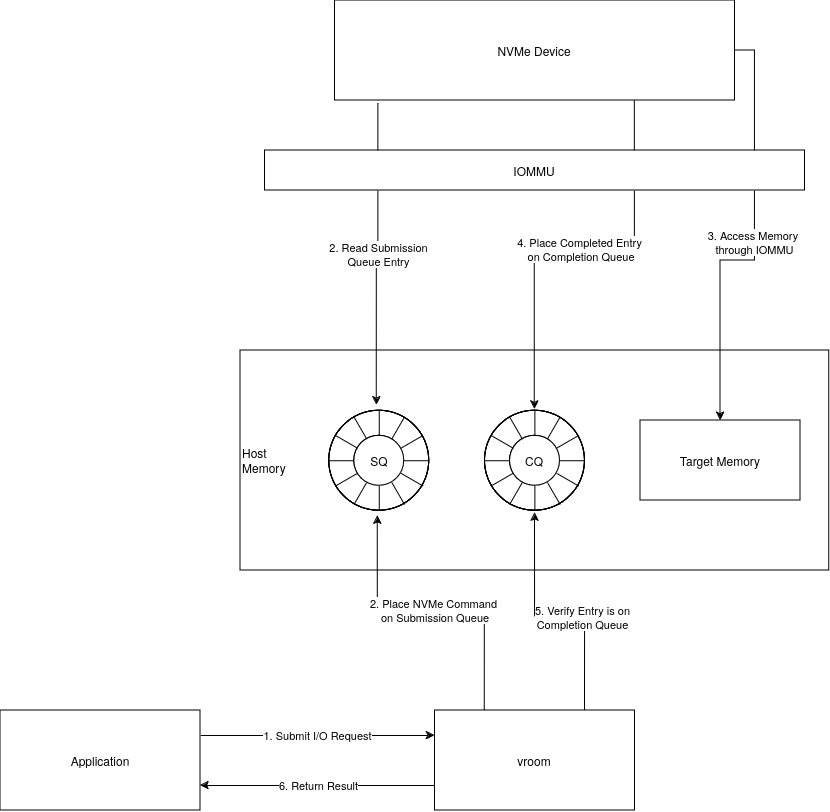
\includegraphics[width=\textwidth]{figures/vroomgraphlight.png}
    \caption{I/O operation vroom}
    \label{fig:vroom-graph}
\end{figure}

\subsection{Initialising the IOMMU}

To use the IOMMU for the driver, we first need to initialize the VFIO kernel module and bind the VFIO driver to the NVMe device:
This has to be done using root privileges. By chowning the VFIO container, the driver can use the VFIO driver to interact with the device without root.

\begin{enumerate}
    \item Add VFIO kernel module using \texttt{modprobe}
    \item Unbind kernel driver from NVMe
    \item Using vendor and device id to bind VFIO to the device
    \item Setting VFIO group permissions to user/group using \texttt{chown}
\end{enumerate}

\begin{lstlisting}[language=bash,caption={Initializing VFIO using bash}]
    #!/bin/bash
    modprobe vfio-pci
    nvme_vd="$(cat /sys/bus/pci/devices/$nvme/vendor) $(cat /sys/bus/pci/devices/$nvme/device)"
    echo $nvme > /sys/bus/pci/devices/$nvme/driver/unbind
    echo $nvme_vd > /sys/bus/pci/drivers/vfio-pci/new_id
    chown $user:$group /dev/vfio/*     
\end{lstlisting}

After this, the real work of the driver happens using these steps:

\begin{enumerate}
    \item Mapping the NVMe device memory into host memory using VFIO resource info.
    \item Allocating Admin SQ, CQ and I/O SQ, CQ
    \item Creating a mapping on the IOMMU using VFIO
    \item Configuring the NVMe device
    \item Passing I/O Queue addresses to NVMe device using admin queues
\end{enumerate}


\subsection{Enabling DMA}

\subsection{Mapping DMA}
In order to provide a section of memory on which the device can perform DMA operations, the user needs to allocate some memory in the processes address space. This is done by using mmap. Using mmap's flags we can also define the page size used. The MAP\_HUGETLB is used in conjunction with the MAP\_HUGE\_2MB and MAP\_HUGE\_1GB flags for 2MiB and 1 GiB pages respectively. By default mmap uses the default page size of 4KiB.
The main IOMMU work is done by then creating the map struct vfio\_iommu\_type1\_dma\_map. We set the DMA mapping to read and write, and provide the same IOVA as the Virtual address. By then passing it to an ioctl call with the according VFIO operation VFIO\_IOMMU\_MAP\_DMA we can create a mapping in the page tables of the IOMMU. This way we can give the IOVA to the NVMe controller, which it will use to access the memory through the address translation of the IOMMU.

\subsection{Unmapping DMA}
Unmapping DMA happens when the process exits, yet for performance and application reasons there is the unmap\_dma function which can be used to unmap a DMA. It is necessary to increase the allocated size to a multiple of the page size as otherwise the munmap operation will result in a failure.

\subsection{Regions}
Using regions, we can directly mmap device memory into host memory for easy access to the NVMe controller.
VFIO provides structs for using mmap to directly map the NVMe device into memory. Using \texttt{VFIO\_DEVICE\_GET\_REGION\_INFO} we can attain the length and the offset needed for mmap.

\subsection{Groups}
VFIO uses group to distinguish between groups of devices which can be isolated from the host system. In the ideal case, every device would only be part of one group in order to increase security by providing single-device isolation. Groups are the smallest unit size on a system to ensure secure user access.

\subsection{Containers}
To further reduce overhead from the IOMMU Containers are used in VFIO, which can hold multiple groups. These containers can be used to ease translation and reduce TLB page faults.
In our implementation we use one group and container each for our NVMe device.

\section{IOMMUFD}
IOMMUFD has only been recently added to the Linux Kernel. E.g. Debian 12 does not support it. In our driver we offer both options of using the IOMMU.
The device file descriptor, which was previously attained with \texttt{VFIO\_GROUP\_GET\_DEVICE\_FD} can now be gotten through opening the character device /dev/vfio/devices/vfioX.
By using this character device pointer we can claim the ownership over the VFIO device. That way VFIO does not rely on group/container/iommu drivers.
As IOMMUFD is not widely used yet, we conducted the evaluation with the legacy VFIO group interface. The performance should not differ, as the hardware is the bottleneck during I/O operations.

\subsection{IOAS}
